\graphicspath{{./communication/}}
\chapter{Arbeitspaket Kommunikation}
Für die Analyse, den Entwurf, die Impelementierung und die Integration dieses Arbeitspaketes übernahm Herr Schleinkofer die Verantwortung.
\paragraph{}
Da die Projektspezifikation einen Datenaustausch zwischen $\mu$-Controller und PC enthält, muss diese auch im Projekt realisiert werden. Dabei können auch Parallelen zum ISO/OSI-Schichtenmodell für Netzwerkkommunikation gezogen werden.
\section{Analysephase}
\subsection{Hardware}
Wie auch in der Physical-Layer behandelt, muss die Kommunikation in diesem Projekt zunächst physikalisch erfolgen. 
Dabei stellt sich die Frage, welche Möglichkeiten der Controller zur Datenübertragung an ein externes Gerät bietet. In dessen Handbuch ist aufgeführt, dass dort ein Universal Serial Interface Channel (USIC) Baustein zur Verfügung steht. Dies würde eine serielle Kommunikationsverbindung über UART ermöglichen. Weitere Möglichkeiten sind auf dem Evaluation Board kaum gegeben. Dieses ist zwar für Ethernet vorbereitet, jedoch müssen dafür ein zusätzlicher Chip und eine RJ45-Buchse nachgerüstet werden. Eine selbst definierte und implementierte parallele Schnittstelle mit den GPIO-Ports wäre theoretisch auch möglich, jedoch in der Umsetzung zu komplex und zeitintensiv.
\paragraph{}
Die gemachten Überlegungen haben zur Folge, dass die Kommunikation zwischen Testplatz und PC über die serielle Schnittstelle abgewickelt wird. Nun muss entschieden werden, welches Gerät am Computer verwendet werden soll. Möglich wäre eine Kommunikation über ein serielles Kabel, welches an eine EIA-232 Schnittstelle des PC's angeschlossen wird. Dies ist jedoch mit einigen Problemen behaftet. Zunächst verfügen moderne Desktop Computer nur noch in wenigen Fällen über eine dedizierte EIA-232 Schnittstelle. Dies kann jedoch durch Verwendung eines USB-zu-Seriell-Adapters umgangen werden. Am $\mu$-Controller erfolgt dann der Anschluss an die GPIO-Pins. Allerdings muss dafür ein Adapter angefertigt werden, welcher auf der einen Seite einen D-Sub 9 Stecker und auf der anderen Seite mindestens die Pins 2 (Data Transceive), 3 (Data Receive) und 5 (Ground) als Stifte, passend zur Buchsenleiste des Evaulation Boards, weiterführt. Allerdings werden die Daten an der EIA-232 Schnittstelle mit bis zu 9 Volt übertragen. Dies stellt ein weiteres Problem dar, da an den Pins des Controllers nur 3,3 Volt ausgegeben werden können. Auch kann ein Eingangssignal mit 9 Volt zu Schäden am $\mu$-Controller führen. Um dieses Problem zu umgehen, wäre es möglich, einen USB-zu-Seriell-Adapter mit integriertem Wandler-Chip zu verwenden.
\paragraph{}
Eine weitere Möglichkeit zur seriellen Kommunikation zeigt ein Beispielprojekt von Infineon für das Evaluation Board auf. In diesem erfolgt die Kommunikation zwischen PC und Controller über das USB-Kabel, welches am Debugging-Chip des Boards angeschlossen wird. Auch in diesem Projekt erfolgt der Datenaustausch mit Nutzung des USIC-Bausteins. Allerdings werden hier die Sende- und Empfangsleitungen an den ... Chip weitergeleitet. Für den PC ist darüber hinaus ein Windows-Treiber verfügbar, welcher einen "virtuellen Com-Port" zur Kommunikation mit dem Evaluation Board einrichtet und über den nun Daten im Rahmen des Beispielprojektes ausgetauscht werden können. Auf die Software des PC's hat diese Vorgehensweise keinen Einfluss, da ein virtueller Com-Port in der gleichen Weise verwendet wird, wie ein Hardware-Gerät. Ein weiterer Vorteil dieser Lösung ist, dass eine zusätzliche Stromversorgung des $\mu$-Controllers entfällt, da dies über das USB-Kabel der Kommunikation erfolgt.
\paragraph{}
Die Aufgaben der zweiten Schicht des ISO/OSI-Modells umfassen unter Anderem auch die Sicherung der Datenintegrität während der Übertragung. Dies geschieht im Fall des Ethernet-Protokolls mittels eines Cyclic Redundancy Check Verfahrens. Und auch andere Kommunikationsprotokolle nutzen diese Art der Integritätsprüfung um etwaigen Störungen während der Übertragung entgegenzuwirken.
\paragraph{}
Weitere Funktionen aus höheren Schichten des ISO/OSI-Modells scheinen in der gegebenen Zeit nicht umsetzbar oder werden schlichtweg nicht benötigt. Eine Adressierung der Kommunikationspartner ist in diesem Fall aufgrund der auf genau zwei beschränkten Anzahl an Kommunikationsteilnehmern genausowenig notwendig wie eine Sitzungsverwaltung ähnlich derer in OSI-Schicht 5. Eine Flusskontrolle oder Empfangsbestätigung ist im Falle zu übertragender Sensordaten auch nicht sinnvoll. Diese Sensordaten sollen nach den Anforderungen regelmäßig vom $\mu$-Controller an den PC gesendet werden. Bei höheren Drehgeschwindigkeiten des Motors würden diese nur unnötig Rechenzeit auf der Senderseite verbrauchen. Bei der Übertragung von Regelungsparametern allerdings könnte eine Empfangsbestätigung durch den $\mu$-Controller durchaus nützlich sein. Allerdings ist hierzu wie bereits erwähnt der Zeitrahmen zu eng gesteckt.
\subsection{Software}
Des weiteren muss noch Analysiert werden, wie die Sensor- und Regelungsdaten für die Kommunikation aufbereitet werden. Hierzu kommen verschiedene Serialisierungsverfahren in Betracht. Zunächst besteht die Möglichkeit die Daten als String zu formatieren und die einzelnen Zeichen als char-Daten seriell zu übertragen. Dies ist eine einfache Lösung, jedoch für zukünftige Änderungen nur schlecht erweiterbar. Es muss dazu für jeden Sensor die komplette Decodierungs-Routine auf beiden Kommunikationspartnern angepasst werden. Sollten nun in Zukunft beispielsweise mehr Experimentierplätze mit unterschiedlichen Sensoren existieren, muss darauf geachtet werden, dass zu jedem auch ein PC verwendet wird, dessen GUI auch den String mit den vorliegenden Sensorwerten auswerten kann.
\paragraph{}
Alternativ dazu kann ein Serialisierungsformat mit dem Namen "Protocol Buffers" (kurz: Protobuf)  verwendet werden. Dieses wurde durch die Firma Google entwickelt und ist für mehrere Programmiersprachen verfügbar. Dies ist wichtig, da die Software auf dem $\mu$-Controller in C, der Teil für den PC aber in C\# geschrieben wird. Der Vorteil dieser Lösung besteht darin, dass etwaige neu hinzukommende Sensoren einfach in die Protobuf-Nachrichten aufgenommen werden können. Kann eine Gegenstelle diesen Teil einer Nachricht nicht verarbeiten, so wird dieser einfach ignoriert.
\paragraph{}
\begin{lstlisting}[caption=Beispieldefinition einer Protocol Buffers Nachricht, label=lst:protoEx]
message Person {
  required string name = 1;
  required int32 id = 2;
  optional string email = 3;
}
\end{lstlisting}
Dies liegt in der Art, wie eine Nachricht in Protobuf aufgebaut ist. Zunächst wird diese in einer Beschreibungssprache definiert.
Im Code \ref{lst:protoEx} ist ersichtlich, dass eine "Message" aus mehreren Feldern und deren zugehörigen Identifiern ("= 1" für das Feld "name") besteht. Wird nun eine Nachricht um neue Felder erweitert, so kann ein Programm, welches jedoch noch die alte Beschreibung nutzt, eine neuartige Nachricht wieder deserialisieren. Die neuen Felder jedoch werden hierbei aufgrund des unbekannten Identifiers ignoriert. Protobuf verfügt darüber hinaus noch über einen Codegenerator. Das bedeutet: Der Entwickler definiert in der gezeigten Beschreibungssprache eine Nachricht. Diese Beschreibung wird nun duch den Generator in einen Code zur De-/Serialisierung umgewandelt. Zusätzlich wird dabei eine Datenstruktur definiert, die vom Entwickler im Programmcode mit den zu übertragenden Daten ausgefüllt werden und einfach in einen Bytestream verwandelt und wieder zurückverwandelt werden kann.
\paragraph{}
Zwar gibt es keine "offizielle" Implementierung von Protobuf für C, jedoch gibt es ein Projekt mit dem Namen "nanopb" welches die grundlegenden Funktionen von Protocol Buffers in C speziell für Embedded Systems umsetzt. Ein weiterer Vorteil von Protobuf gegenüber der einfachen String-Variante ist die geringere Größe der einzelnen Nachrichten, was die Kommunikation effizienter werden lässt.
\section{Entwurfsphase}
Der Ablauf der Kommunikation sollte relativ einfach gehalten werden, um in der vorgegebenen Zeit umsetzbar zu sein. Daher senden die Kommunikationspartner nur einfache Protobuf-Nachrichten. Der PC sendet Regelungsparameter und Ziel an den Controller. Dieser wiederum sendet regelmäßig die Daten der angeschlossenen Sensoren an die GUI auf dem PC. Um die Kommunikation für die angrenzenden Arbeitspakete so einfach wie möglich zu gestalten, soll die Schnittstelle nur aus wenigen Funktionen bzw. Methoden bestehen.
\subsection{Nachrichtendefinition}
Im System gibt es zwei Arten von Nachrichten. Die erste Art enthält die gesammelten Daten aller Sensoren auf dem Controller und wird von diesem an den PC verschickt. Die zweite Art enthält die Regelungsparameter und die Größe, welche geregelt werden soll. Diese Parameter können an der GUI eingestellt und an den $\mu$-Controller gesendet werden. Der grundlegende Aufbau beider Nachrichten auf Byte-Ebene ist gleich und wird in Bild \ref{fig:FrameOv} dargestellte. Den Beginn der Nachricht markiert ein Byte, welches die Anzahl aller Bytes der Nachricht (nachfolgend Frame genannt) enthält. Anschließend folgen die bereits von Protobuf serialiserten Daten als Reihe von Bytes. Den Abschluss des Frames bilden zwei Bytes, welche die CRC Prüfsumme enthalten. Bei der Prüfsumme handelt es sich um die 16-Bit große CRC-CCITT, welche unter anderem auch beim seriellen Datenübertragungsprotokoll HDLC verwendet wird.
\begin{figure}[h]
  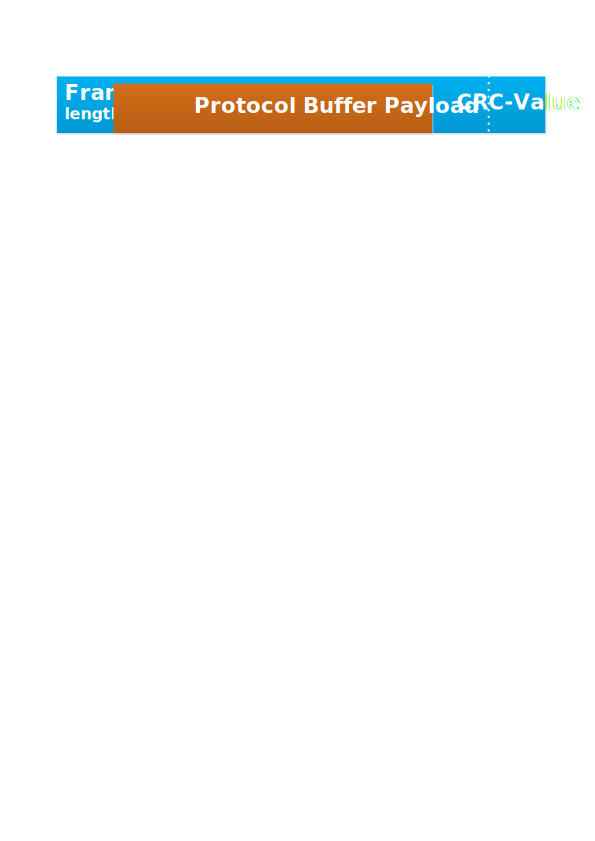
\includegraphics[width=\textwidth]{MessageFormat}
  \caption{Schematischer Aufbau eines Frames}
  \label{fig:FrameOv}
\end{figure}
\subsubsection{Sensordaten Nachricht}
Bei der Absprache mit den für die GUI verantwortlichen Entwicklern, kam folgende Anforderung hinzu: "Die Nachrichten sollen mit einem Zeitstempel oder einer fortlaufenden Nummer ausgestattet sein, um diese später unter Umständen nochmals sortieren zu können." Um auch für zukünftige Erweiterungen von Sensoren gerüstet zu sein, soll die Anzahl der Sensordaten in der Nachricht variabel gestaltet sein. Zudem wird jedem Sensorwert die ID des Sensors, welcher den Wert produzierte, zugeordnet. Um das alles zu erfüllen gilt für die Protobuf Nachricht folgende Beschreibung:
\begin{lstlisting}[caption=Beschreibung der Sensordaten Nachricht, label=lst:protoData]
//defining an entry of the data table
message DataEntry{
	uint32 SensorId = 1;
	double Data = 2;
}
//defining the real message
message SensorMsg{
	//Upcounting Nr
	uint64 SequenceNr = 1;
	//all Data
	repeated DataEntry DataTable = 2;
}
\end{lstlisting}
\subsubsection{Regelungsparameter Nachricht}
Das Team, welches die Regelung umgesetzt hat, stellt eine API bereit, welche neben den Parametern P, I und D eines Reglers auch die Regelgröße (z.B. Geschwindigkeit oder Drehmoment) und den Zielwert entgegennimmt. Dazu müssen diese Werte auch in der Protobuf Nachricht wie folgt berücksichtigt werden:
\begin{lstlisting}[caption=Beschreibung der Parameter Nachricht, label=lst:protoPara]
//defining the parameter message
message RegParams{
	uint32 target = 1;
	float paraP = 2;
	float paraI = 3;
	float paraD = 4;
	float tgtVal = 5;
}
\end{lstlisting}
Im Codebeispiel \ref{lst:protoPara} wird die Regelgröße mittels dem "target" Feld übermittelt. Dabei muss jedoch beachtet werden, dass bei beiden Kommunikationspartnern die Werte der gleichen Größe zugeordnet werden.
\paragraph{PC Bibliothek}
Für den Teil, welcher die Kommunikation auf Seiten der GUI übernimmt, soll eine Bibliothek auf C\#-Basis implementiert werden. Um nun Regelungsparameter an den Controller senden zu können, muss ein Datenobjekt beim Aufruf der Sende-Methode übergeben werden. Für den Empfang von Sensordaten ist es von Vorteil, das Hollywood-Prinzip anzuwenden. So soll die Bibiliothek nicht regelmäßig nach neuen Daten abgefragt werden. Vielmehr lößt die API ein Event aus, welches die Verfügbarkeit neuer Werte anzeigt. Da sich bereits darauf festgelegt wurde, einen virtuellen Com-Port zur Kommunikation zu verwenden, soll dieser nun auch bei der Initialisierung der API als String oder gleich als ComPort-Objekt mit angegeben werden. 
\paragraph{Controller Funktionen}
\section{Implementierung}
\section{Integration}
\section{Ausblick}
